\documentclass[a4paper,12pt]{article}

\usepackage{mystyle}

\usepackage{gensymb}
\usepackage{scalerel}
\usepackage{stackengine}

% \usepackage{skull}  % skull
\usepackage{halloweenmath}  % \bigpumpkin, skull (https://tug.ctan.org/info/symbols/comprehensive/symbols-a4.pdf -- Table 76)


% https://tex.stackexchange.com/questions/3266/how-do-i-use-a-circle-as-a-math-accent-larger-than-mathring
% https://tex.stackexchange.com/a/3270/135045
\usepackage{accents}

\renewcommand{\mathring}[1]{\accentset{\circ}{#1}}


\graphicspath{ {images/} }


% https://tex.stackexchange.com/questions/5461/is-it-possible-to-change-the-size-of-an-arrowhead-in-tikz-pgf
\usetikzlibrary{arrows.meta}


\DeclareMathOperator{\Image}{Im}

\definecolor{pink}{RGB}{218, 3, 174}
\definecolor{violet}{RGB}{148, 0, 211}
\definecolor{green}{RGB}{0, 153, 0}
\definecolor{orange}{RGB}{255, 153, 0}
\definecolor{blue}{RGB}{5, 73, 255}
\definecolor{cyan}{RGB}{31, 206, 203}
\definecolor{cyan2}{RGB}{0, 166, 147}
\definecolor{cyangreen}{RGB}{0, 155, 118}
\definecolor{cyangreen2}{RGB}{0, 109, 91}


% https://tex.stackexchange.com/a/101138/135045

\newcommand\widesim[1]{\ThisStyle{%
  \setbox0=\hbox{$\SavedStyle#1$}%
  \stackengine{-.1\LMpt}{$\SavedStyle#1$}{%
    \stretchto{\scaleto{\SavedStyle\mkern.2mu\sim}{.5150\wd0}}{.6\ht0}%
  }{O}{c}{F}{T}{S}%
}}


\newcommand{\BigMiddleThree}{\;\left|\vphantom{\begin{pmatrix} 0\\0\\0 \end{pmatrix}}\right.\;}
\newcommand{\BigMiddleFour}{\;\left|\vphantom{\begin{pmatrix} 0\\0\\0\\0 \end{pmatrix}}\right.\;}


% https://tex.stackexchange.com/questions/63531/how-to-write-quotation-marks-in-math-environment
\DeclareMathSymbol{\mlq}{\mathord}{operators}{``}
\DeclareMathSymbol{\mrq}{\mathord}{operators}{`'}


\DeclareMathOperator{\Imag}{Im}


% https://tex.stackexchange.com/questions/544453/undefined-control-sequence-after-paragraph
\renewcommand{\paragraph}[1]{\noindent\textbf{#1}\quad}


% https://tex.stackexchange.com/questions/36851/skipping-line-after-proof-in-proof-environment#comment73553_36851
\newcommand{\proofindent}{\hspace*{\fill}\par\vspace{0.5em}\noindent}


% https://tex.stackexchange.com/questions/4813/extendible-equals-sign
\makeatletter
\newcommand*{\Relbarfill@}{\arrowfill@\Relbar\Relbar\Relbar}
\newcommand*{\xeq}[2][]{\ext@arrow 0055\Relbarfill@{#1}{#2}}
\makeatother


% https://tex.stackexchange.com/questions/279100/typeset-the-shrug-%C2%AF-%E3%83%84-%C2%AF-emoji
\newcommand{\shrug}[1][]{%
\begin{tikzpicture}[baseline,x=0.8\ht\strutbox,y=0.8\ht\strutbox,line width=0.125ex,#1]
  \def\arm{(-2.5,0.95) to (-2,0.95) (-1.9,1) to (-1.5,0) (-1.35,0) to (-0.8,0)};
  \draw \arm;
  \draw[xscale=-1] \arm;
  \def\headpart{(0.6,0) arc[start angle=-40, end angle=40,x radius=0.6,y radius=0.8]};
  \draw \headpart;
  \draw[xscale=-1] \headpart;
  \def\eye{(-0.075,0.15) .. controls (0.02,0) .. (0.075,-0.15)};
  \draw[shift={(-0.3,0.8)}] \eye;
  \draw[shift={(0,0.85)}] \eye;
  % draw mouth
  \draw (-0.1,0.2) to [out=15,in=-100] (0.4,0.95); 
\end{tikzpicture}}



% https://tex.stackexchange.com/a/314638/135045
\newcommand{\diff}{\mathop{}\!d\!}



\author{Алексеев Василий}


\title{Семинар 4 + 5}
\date{23 + 30 сентября 2024}


\begin{document}
  \maketitle
  
  \tableofcontents

  \thispagestyle{empty}
  
  \newpage
  
  
  
  \vspace*{\fill}
  
  \noindent
  \emph{
    К формулировкам и доказательствам (если такие вообще приводятся) стоит относиться критически.
    Основное в этом конспекте~---~решение задач (но ``критичность'' и здесь лучше не отключать).
    За строгой, ясной и последовательной теорией лучше обращаться к ``нормальным'' источникам.
    (Например, к лекциям.)
  }
  
  \vspace*{\fill}
  
  \thispagestyle{empty}
  
  \newpage
  
  
  \pagenumbering{arabic}


  % \section{Функции}
  
  %\begin{figure}[ht]
    %\centering
    %\includegraphics[width=0.6\linewidth]{images/Apples}
    %
    %\caption{
      %Одно яблоко, два яблока, ...~---~натуральные числа используются при счёте предметов.
    %}
    %\label{fig:naturals}
  %\end{figure}

  % TODO: про инъективность, сюръективность
  % https://github.com/Alvant/GeomeSeminare/tree/master2022/seminars/linalge/seminar05
  
  

  \section{Предел функции}

  При разговоре о производной функции в точке~$x_0$ было важно, как \emph{меняется} функция в окрестности точки~---~смотрели на разницу значений функции $f(x) \hm- f(x_0)$ для ``близких'' к~$x_0$ точек~$x$.
  (По сути производная и показывает скорость изменения.)
  Получается, для существования вообще производной функии~$f(x)$ в точке~$x_0$ функция должна быть определена в некоторой $U_{\delta}(x_0)$ окрестности этой точки, включая саму точку.

  Но можно ещё задаться таким вопросом: как \emph{ведёт} себя функция в окрестности точки?
  какие значения принимает функция в ``близких'' к~$x_0$ точках~$x$?
  Для всех ``нормальных'' функций, очевидно, ожидается, что по мере приближения $x$ к $x_0$ будет наблюдаться и сближение $f(x)$ с $f(x_0)$.
  Но всегда ли так будет происходить?
  Да и вообще: ведь \emph{не важно значение функции в самой точке~$x_0$}, чтобы понять, как она ведёт себя в её окрестности? (приближается ли $f(x)$ к чему-то вообще или нет)
  Это поведение функции при приближении к точке~$x_0$ описывается понятием \emph{предела функции в точке}.
  Получается, для существования предела функции~$f(x)$ в точке~$x_0$ функция должна быть определена в некоторой $U_{\delta}(x_0)$ окрестности этой точки, \emph{исключая, возможно, саму точку}~---~то есть важна окрестность без ``центральной'' точки, или \emph{проколотая окрестность} точки:
  \[
    \mathring U_{\delta}(x_0) \hm\equiv U_{\delta}(x_0) \hm\setminus \{x_0\} = \{x\colon 0 \hm< |x \hm- x_0| \hm< \delta\}
  \]
  % TODO: картинки про "смысл" предела в точке

  Существует два подхода к ``формализации'' описания того, что значит ``поведение функции~$f(x)$ при приближении $x$ к $x_0$''...
  (При этом суть за обоими подходами одинаковая~---~кусочек графика функции лежит в квадратике около некоторой точки с абсциссой~$x_0$, как бы сильно этот квадратик ни уменьшать~\ref{fig:squares}).
  
  \begin{figure}[ht]
    \centering
    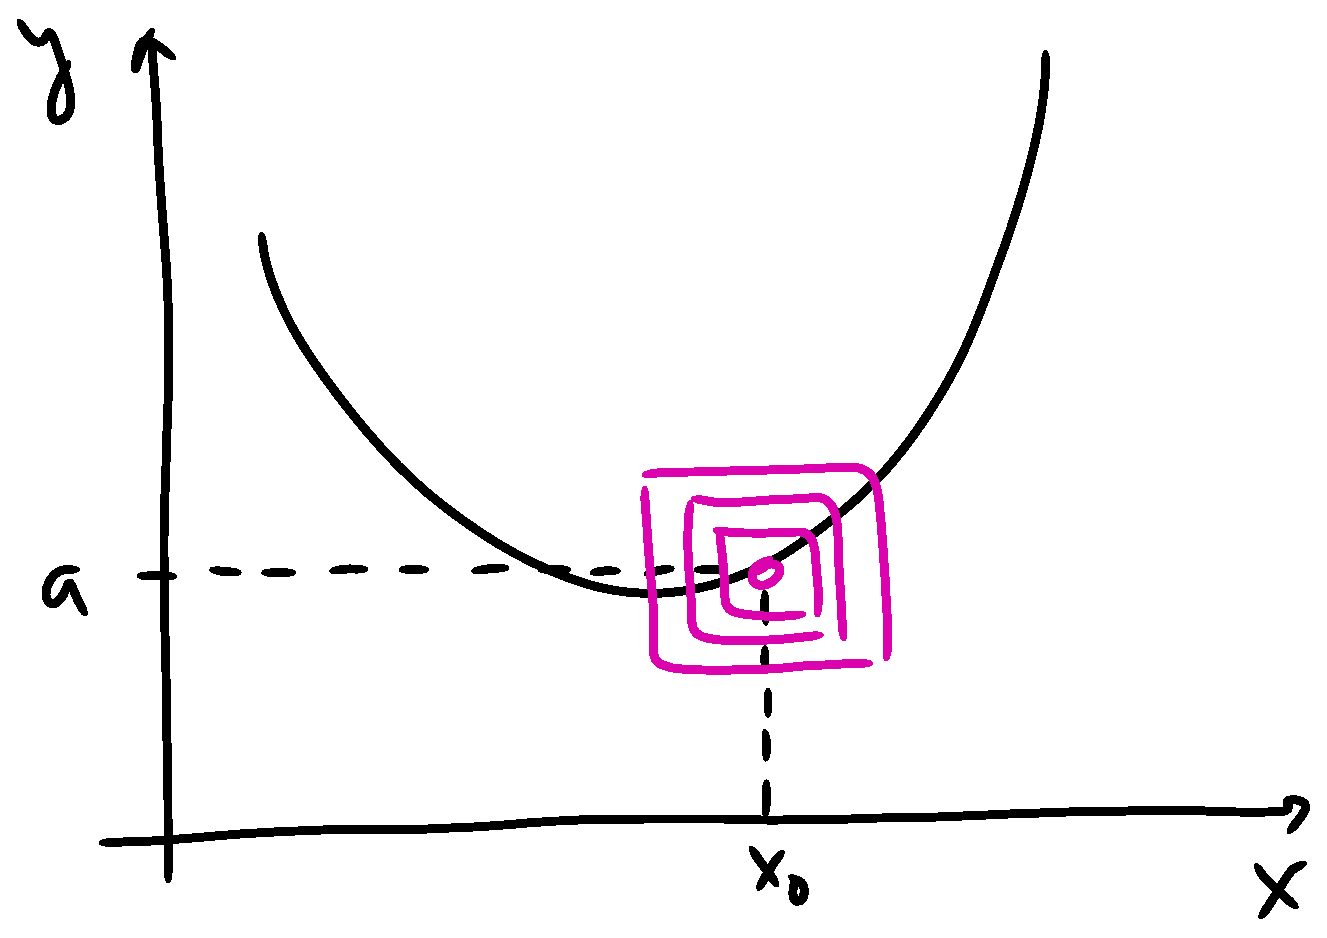
\includegraphics[width=0.6\linewidth]{images/squares}
    
    \caption{
      Предел функции в точке~---~чем ближе по оси $X$ точки $x$ к $x_0$, тем ближе по оси $Y$ значения $f(x)$ к $a$.
    }
    \label{fig:squares}
  \end{figure}


  \subsection{Определения предела функции}
  
  \begin{definition}[Предел по Коши]
    Пусть функция~$f(x)$ определена в некоторой проколотой $\mathring \delta_0$-окрестности точки~$x_0$.

    Элемент~$a \hm\in \RR \hm\cup \{\pm \infty, \infty\}$ (число или какая-то бесконечность) называется \emph{пределом} функции в точке~$x_0 \hm\in \RR \hm\cup \{\pm \infty, \infty\}$ в смысле Коши, если
    \begin{equation}\label{eq:koshi}
      \forall \eps > 0\ \exists \delta > 0\colon \forall x \in \mathring U_{\delta}(x_0) \to f(x) \in U_{\eps}(a)
    \end{equation}

    Если и $x_0$, и $a$~---~это просто числа, то можно написать и так:
    \[
      \forall \eps > 0\ \exists \delta > 0\colon \forall x\colon 0 < |x - x_0| < \delta \to |f(x) - a| < \eps
    \]
  \end{definition}

  \begin{definition}[Предел по Гейне]
    Пусть функция~$f(x)$ определена в некоторой проколотой $\mathring \delta_0$-окрестности точки~$x_0$.

    Элемент~$a \hm\in \RR \hm\cup \{\pm \infty, \infty\}$ (число или какая-то бесконечность) называется \emph{пределом} функции в точке~$x_0 \hm\in \RR \hm\cup \{\pm \infty, \infty\}$ в смысле Гейне, если  % TODO: check inftys
    \begin{equation}\label{eq:giyne}
      \forall \{x_n\}_{n=1}^{\infty}\colon \left\{
        \begin{aligned}
          &\lim_{n \to \infty} x_n = x_0\\
          &x_n \not{=} x_0,\ \forall n \in \NN
        \end{aligned}
      \right.
      \to \lim_{n \to \infty} f(x_n) = a
    \end{equation}
    где описанная последовательность $\{x_n\}_{n=1}^{\infty}$ называется \emph{последовательностью Гейне} в точке~$x_0$ (то есть это такая последовательность, которая сходится к~$x_0$, при этом в саму~$x_0$ никогда не попадая).
  \end{definition}

  \begin{remark}
    Проколотость окрестности около точки~$x_0$ в определении предела по Коши, условие $x_n \hm{\not=} x_0$ в определении предела по Гейне~---~всё это выражение того, что для предела функции в точке не важно, что происходит с функцией в самой точке~---~важно лишь её поведение вблизи точки.
  \end{remark}

  Два определения (пусть и с похожей идеей)~---~по-хорошему, стоило бы предположить, что они, возможно, определяют разные понятия: что может быть предел~$a$ функции в точке~$x_0$ по Коши, но это не будет пределом по Гейне, или наоборот.
  Но ``оказывается'', что два определения предела \emph{равносильны}, взаимозаменяемы.
  Из одного следует другое, и наоборот.
  Покажем это...

  \begin{proof}[Коши $\to$ Гейне]
    Считаем, что~$a$ есть предел функции $f(x)$ в точке $x_0$ в смысле Коши~\eqref{eq:koshi}.
    Надо показать, что $a$ будет и пределом в той же точке по Гейне~\eqref{eq:giyne}.

    То есть надо доказать, что ``для \emph{любой} последовательности Гейне...''
    Как это сделать?
    Все-все последовательности Гейне в точке, очевидно, перебрать не сможем.
    Но можно взять \emph{произвольную} последовательность Гейне в точке~$x_0$ и доказать всё для неё.
    Или можно допустить, что \emph{найдётся хотя бы одна} последовательность Гейне, для которой условие предела по Гейне выполняться не будет, и попробовать получить отсюда какое-нибудь противоречие (с тем, что~$a$ есть предел по Коши).
    Второй способ~---~способ от противного.
    Пойдём по нему.
    То есть допускаем отрицание~\eqref{eq:giyne}: найдётся последовательность Гейне $\{x_n\}_{n=1}^{\infty}$ в точке~$x_0$, такая что предела $\lim_{n \to \infty} f(x_n)$ не существует, либо $\lim_{n \to \infty} f(x_n) \hm{\not=} a$.
    Почему это ``плохо''?
    Это может противоречить тому, что про $a$ известно, что это~---~предел по Коши.
    То есть отсюда можно выйти на отрицание условия Коши~\eqref{eq:koshi} предела...\footnote{
      Забавно.
      Идём по от-противным, сначала отрицание ``по Гейне'', теперь ``по Коши''.
    }
    \[
      \exists \eps > 0\colon \forall \delta > 0\ \exists x \in \mathring U_{\delta}(x_0)\colon f(x) \not\in U_{\eps}(a)
    \]

    Почему при наличии ``нехорошей'' последовательности Гейне~$\{x_n\}_{n=1}^{\infty}$ верно отрицание Коши?
    Потому что ``нехорошесть''$\{x_n\}_{n=1}^{\infty}$~---~она по сути означает то же самое, что и отрицание Коши!
    (Читателю рекомендуется сделать здесь паузу, чтобы ``прочувствовать и осознать''.)
    Для строгости и понятности изложения, поясним идею более конкретно, не на словах.
    Ещё раз: последовательность Гейне~$\{x_n\}_{n=1}^{\infty}$ сходится к~$x_0$, то есть:
    \[
      \forall \delta > 0\ \exists N(\delta) \in \NN\colon \forall n \geq N(\delta) \to x_n \in \mathring U_{\delta}(x_0)
    \]
    но $\{f(x_n)\}_{n = 1}^{\infty}$ при этом к $a$ не сходится, то есть:
    \[
      \exists \eps > 0\colon \forall \widetilde N(\eps) \in \NN\ \exists n(\eps, \widetilde N) \geq \widetilde N\colon f(x_n) \not\in U_{\eps}(a)
    \]
    (где выражением $\exists n(\eps, \widetilde N)$ подчёркнуто, что этот номер $n$ зависит от обозначенных ранее в том же условии $\eps$ и $\widetilde N$~---~то есть выбор этого $n$ есть по сути \emph{функция} от $\eps$ и $\widetilde N$ (ну, и вообще, конечно, можно ещё считать $n$ функцией только $\eps$, ведь $\widetilde N$ тоже определяется $\eps$...)).
    Объединяя два в одном, получаем:
    \[
      \exists \eps > 0\colon \forall \delta > 0\ \exists x = x_{n(\eps, N(\eps))} \in \mathring U_{\delta}(x_0)\colon f(x) \not\in U_{\eps}(a)
    \]
    что уже просто один-в-один совпадает с отрицанием Коши равенства~$a$ предела функции~$f(x)$ в точке~$x_0$.
  \end{proof}

  \begin{proof}[Гейне $\to$ Коши]
    Теперь, наоборот, считаем, что~$a$ есть предел функции $f(x)$ в точке $x_0$ в смысле Гейне~\eqref{eq:giyne}.
    Надо показать, что $a$ будет и пределом в той же точке по Коши~\eqref{eq:koshi}.

    Опять, есть два пути.
    Можно взять \emph{произвольное} $\eps \hm> 0$ и убедиться, что для него найдётся $\delta \hm> 0$, такой что... (и так далее по определению предела в точке в смысле Коши)~---~таким образом доказав ``предельность'' по Коши для всех $\eps \hm> 0$.
    А можно~---~допустить, что \emph{найдётся хотя бы одно} $\eps > 0$, для которого ``предельность'' по Коши верна не будет, и как-нибудь из этого получить противоречие.
    Таким образом доказав ``предельность'' по Коши от противного.

    Продолжим ``путь по от-противным''.

    Допустим, что $a$ \textbf{не} будет пределом в~$x_0$ по Коши~\eqref{eq:koshi}, то есть что будет верно отрицание ``предельности'' по Коши:
    \begin{equation}\label{eq:neg-koshi}
      \exists \eps > 0\colon \forall \delta > 0\ \exists x \in \mathring U_{\delta}(x_0)\colon f(x) \not\in U_{\eps}(a)
    \end{equation}

    Как из этого получить противоречие?
    По аналогии с предыдущим доказательством~---~получим противоречие с тем, что начали-то с верности ``предельности'' по Гейне.
    То есть надо как-то выйти на \emph{отрицание} того, что $a$ есть предел в~$x_0$ по Гейне~\eqref{eq:giyne}: найдётся последовательность Гейне $\{x_n\}_{n=1}^{\infty}$ в точке~$x_0$, такая что предела $\lim_{n \to \infty} f(x_n)$ не существует, либо он не равен~$a$.\footnote{
      Строчка с отрицанием Гейне скопирована из предыдущего доказательства (где тоже отрицался Гейне, только где это было ``первым'' отрицанием, которое ``от противного'', а не вторым, которое ``для противоречия'').
    }
    Построим же эту последовательность~(\ref{fig:tube})!
    Возьмём некоторый $\delta_1$ (такой чтоб функция~$f$ была определена в $\delta_1$-окрестности~$x_0$).
    Из верности отрицания Коши (``от противного''~\eqref{eq:neg-koshi})~---~найдётся $x_1 \hm\in \mathring U_{\delta_1}(x_0)$, такой что $f(x_1) \hm{\not\in} U_{\eps}(a)$.
    Далее, продолжаем процесс так: $\delta_2 \hm= \frac{\delta_1}{2}$, $x_2 \hm\in \mathring U_{\delta_2}(x_0)$ ($f(x_2) \hm{\not\in} U_{\eps}(a)$), и так далее: уменьшаем $\delta_{n - 1}$-окрестность около~$x_0$ в несколько раз, выбираем из новой окрестности новый $x_n$ (отличный от всех выбранных до этого $x_1$, $x_2$, ..., $x_{n - 1}$), такой чтоб $f(x_n)$ было на расстоянии $\eps$ от $a$ или ещё дальше.
    Получаются последовательности $\{x_n\}$ и $\{f(x_n)\}$.
    Для первой имеем:
    \[
      0 < |x_n - x_0| < \delta_n = \frac{\delta_1}{2^{n - 1}} \xrightarrow{n \to\infty} 0
    \]
    то есть $\{x_n\}$~---~в самом деле последовательность Гейне в точке~$x_0$.
    Но последовательность из значений функций $\{f(x_n)\}$ к~$a$, очевидно, не сходится (на расстоянии $\eps$ от~$a$ нет вообще ни одного члена последовательности $\{f(x_n)\}$).
    Противоречие.
    
    \begin{figure}[ht]
      \centering
      \includegraphics[width=0.6\linewidth]{images/tube}
    
      \caption{
        ``$\eps$-трубка'' вокруг $a$.
      }
      \label{fig:tube}
    \end{figure}
  \end{proof}


  \subsection{Односторонние пределы}

  % TODO: pictures

  При нахождении предела функции в точке~$x_0$ ``двигаемся'' всё ближе к~$x_0$, глядя на значения~$f(x)$.
  Но приближаться к~$x_0$ можно по-разному.
  Так, можно приближаться к ней \emph{слева} или \emph{справа}.
  Двигаясь таким образом, находясь всегда с одной стороны от~$x_0$, приходим к понятию \emph{односторонних} пределов.
  Сформулируем это точнее.
  
  Число или бесконечность $a$ называется \emph{пределом слева} функции $f$ в числовой точке~$x_0$, если:
  \[
    \forall \eps > 0\ \exists \delta > 0\colon \forall x\colon \textcolor{pink}{x_0 - \delta < x < 0} \to f(x) \in U_{\eps}(a)
  \]
  (то есть как предел по Коши~\eqref{eq:koshi}, только находимся всегда в левой половинке $\mathring U_{\delta}(x_0)$).\footnote{
    У окрестностей бесконечностей со знаком $\pm \infty$, видимо, ``половинок'' нет.
    Но половинки есть у окрестности ``просто бесконечности'' $\infty$...
    Получается, можно говорить о пределе слева при $x \hm\to \infty$?..
    (И это будет предел как при $x \hm\to -\infty$?..)
  }
  Или, если смотреть на предел как Гейне~\eqref{eq:giyne}, то левый односторонний предел функции~$f$ в~$x_0$ есть~$a$, если
  \[
    \forall \{x_n\}_{n=1}^{\infty}\colon \left\{
      \begin{aligned}
        &\lim_{n \to \infty} x_n = x_0\\
        &x_n \textcolor{pink}{{}<{}} x_0,\ \forall n \in \NN
      \end{aligned}
    \right.
    \to \lim_{n \to \infty} f(x_n) = a
  \]
  то есть когда все элементы последовательности Гейне находятся ``слева'' от~$x_0$.

  Аналогично определяется предел справа функции~$f$ в~$x_0$.

  Обозначаются левый и правый пределы так:
  \[
    \begin{aligned}
      &\lim_{x \to x_0 - 0} f(x) = f(x - 0) & &\mbox{(левый)}\\
      &\lim_{x \to x_0 + 0} f(x) = f(x + 0) & &\mbox{(правый)}
    \end{aligned}
  \]

  Кажется понятным, что если существует ``просто'' предел функции~$f$ в~$x_0$, то существуют также и левый и правый пределы в той же точке, и они равны ``просто'' пределу.

  Но верно и обратное: если существуют и равны оба односторонних предела в~$x_0$, то существует и ``просто'' предел (и равен односторонним).
  Это тоже, вроде бы, понятно...
  Правда, тут уже, кажется, стоит всё-таки привести какие-то более строгие пояснения.
  Итак, что значит, что существуют односторонние пределы и что они равны (и равны некоторому~$a$):
  \[
    \left\{\begin{aligned}
      &\forall \eps > 0\ \exists \delta > 0\colon \forall x\colon \textcolor{pink}{x_0 - \delta < x < 0} \to f(x) \in U_{\eps}(a)\\
      &\forall \eps > 0\ \exists \delta > 0\colon \forall x\colon \textcolor{pink}{0 < x < x_0 + \delta} \to f(x) \in U_{\eps}(a)
    \end{aligned}\right.
  \]
  (смотрели на пределы как Коши~---~можно бы было и по Гейне).
  Но просто ``объединяя'' вместе эти условия, и получаем, что~$a$ есть ``просто'' предел!
  (Из половинок окрестностей складывается целая (но проколотая) окрестность.)


  \subsection{Замечательные пределы}

  Существуют два ``интересных'' (необычных, важных, удивительных~---~замечательных) предела функций в точке.
  Приведём их без доказательства.

  \begin{proposition}[Первый замечательный предел]
    \begin{equation}\label{eq:first-marvelous}
      \lim_{x \to 0} \frac{\sin x}{x} = 1
    \end{equation}
  \end{proposition}

  \begin{proposition}[Второй замечательный предел]
    \begin{equation}\label{eq:second-marvelous}
      \lim_{x \to 0}\, (1 + x)^{\frac{1}{x}} = e
    \end{equation}
  \end{proposition}

  Без доказательства, но с попыткой осмыслить...

  \begin{remark}[``Попытка принять'']
    Функция под первым замечательным пределом:
    \[
      f(x) = \frac{\sin x}{x}
    \]
    Что можно про неё заметить?
    Во-первых, при $x_0 \hm= 0$ и числитель $\sin x$, и знаменатель обращаются в ноль (отсюда и интересность предела).
    Кроме этого, посмотрим на производные числителя и знаменателя в нуле:
    \[
      (\sin x)'|_{x = 0} = \cos 0 = 1,\quad x'|_{x = 0} = 1
    \]
    то есть производные тоже равны!
    Что получается: $\sin x$ и $x$ равны в нуле, и изменяются одинаково в окрестности нуля (бесконечно малой).
    Таким образом, в этой малой окрестности нуля функции $\sin x$ и $x$ получаются равными!
    (Стартуют из одной точки, и, изменяясь одинаково, приходят снова в одну точку.)
    % TODO: picture
    \medskip

    Теперь посмотрим на второй замечательный предел...\footnote{
      Сразу возникает вопрос, откуда там вообще $e$)
    }
    Что можно бы было с ним сделать, если бы стояла задача найти его?
    \[
      \lim_{x \to 0} (1 + x)^{\frac{1}{x}} = \?
    \]
    Функция под пределом~---~это сложная функция, в табличных такой нет.
    При вычислении производных от функций такого вида можно было преобразовать выражение так, чтобы получилась показательная (с которой уже понятно, что делать).
    Воспользуемся таким же приёмом:
    \[
      \lim_{x \to 0} (1 + x)^{\frac{1}{x}}
        = \lim_{x \to 0} e^{\ln{(1 + x)} \frac{1}{x}}
    \]

    Посмотрим, к чему стремится показатель:
    \[
      \lim_{x \to 0} \frac{\ln{(1 + x)}}{x} = \?
    \]

    % TODO: picture
    Что можно сказать про функцию под пределом?
    (Проведём по пунктам то же ``исследование'', что и при рассмотрении первого замечательного предела.)
    Числитель и знаменатель равны в нуле:
    \[
      \ln{(1 + x)}|_{x = 0} = \ln{1} = 0 = x|_{x = 0}
    \]
    И их производные~---~тоже равны в нуле:
    \[
      \bigl(\ln{(1 + x)}\bigr)'|_{x = 0} = \left.\frac{1}{1 + x}\right|_{x = 0} = 1 = x'|_{x = 0}
    \]
    Получается, равны в начале, изменяются одинаково~---~а потому равны в конце, вблизи нуля, бесконечно близко к нулю, то есть верно соотношение:\footnote{
      Подчеркнём ещё раз, что это не строгое доказательство.
      Можно сказать, что это... немного рукомахательное доказательство, основанное на здравом смысле (и с претензией на понятность и доступность).
    }
    \[
      \lim_{x \to 0} \frac{\ln{(1 + x)}}{x} = 1
    \]
    А потому верно и следующее:
    \[
      \lim_{x \to 0} e^{\frac{\ln{(1 + x)}}{x}} = e^1 = e
    \]

    \medskip

    Хочется верить, что приведённое рассуждение помогло читателю, хоть и не доказать, но, по крайней мере, ``принять'' для себя эти замечательные пределы.
    (Убрать из ``замечательности'' компоненту ``удивительности''.)
  \end{remark}


  \subsection{Эквивалентность функций}

  Если, как в первом замечательном приделе~\eqref{eq:first-marvelous}, отношение двух функций в пределе в некоторой точке~$x_0$ равно единице, то такие функции называются \emph{эквивалентными} при $x \hm\to x_0$:
  \[
    f(x) \sim g(x) \mbox{ при } x \to x_0
      \quad\leftrightarrow\quad \lim_{x \to x_0} \frac{f(x)}{g(x)} = 1
  \]

  \begin{example}
   Кроме $\sin x$ и $x$ при $x \hm\to 0$, эквивалентными будут, например, $x + 1$ и $x + 100$ при $x \hm\to \infty$.
  \end{example}

  Ещё один особый случай отношения между двумя функциями в пределе в некоторой точке~---~когда это отношение $\frac{f(x)}{g(x)}$ равно нулю при $x \hm\to x_0$.
  Тогда говорят, что функция $f(x)$ является $o$-малой относительно $g(x)$ при $x \hm\to x_0$:\footnote{
    $o$-малая от $g(x)$~---~не одна функция, а семейство функций.
  }
  \[
    f(x) = o\bigl(g(x)\bigr) \mbox{ при } x \to x_0
      \quad\leftrightarrow\quad \lim_{x \to x_0} \frac{f(x)}{g(x)} = 0
  \]

  \begin{example}
    Например, $1 \hm= o(x)$ при $x \hm\to \infty$, $1000x^3 \hm= o\left(x^2\right)$ при $x \hm\to 0$.
  \end{example}

  Между эквивалентностью и ``$o$-малостью'' существует связь...

  \begin{proposition}
      Две функции эквивалентны при $x \hm\to x_0$ тогда и только тогда, когда одна из них представима как другая плюс $o$-малая от неё при $x \hm\to x_0$:
      \[
        f(x) \sim g(x) \mbox{ при } x \to x_0
          \quad\leftrightarrow\quad f(x) = g(x) + o\bigl(g(x)\bigr) \mbox{ при } x \to x_0
      \]
  \end{proposition}

  \begin{proof}
      Достаточность ($\Leftarrow$) кажется очевидной.
      Убедимся:
      \[
        f(x) = g(x) + o\bigl(g(x)\bigr) \mbox{ при } x \to x_0
          \rightarrow \frac{f(x)}{g(x)} = 1 + o(1) \mbox{ при } x \to x_0
          \leftrightarrow \lim_{x \to x_0} \frac{f(x)}{g(x)} = 1
      \]

      Покажем необходимость ($\Rightarrow$).
      Имеем:
      \[
        f(x) \sim g(x) \mbox{ при } x \to x_0
          \leftrightarrow \lim_{x \to x_0} \frac{f(x)}{g(x)} = 1
      \]
      то есть для любого (даже сколь угодно малого) $\eps \hm> 0$ в некоторой $\delta$-окрестности $x_0$ будет верно, что
      \[
        1 - \eps < \frac{f(x)}{g(x)} < 1 + \eps
      \]

      ...Сделаем по-другому.
      Откатимся назад:
      \[
        \lim_{x \to x_0} \frac{f(x)}{g(x)} = 1
      \]
      Воспользуемся приёмом ``вычесть и добавить'':
      \[
        \lim_{x \to x_0} \frac{f(x)}{g(x)}
          = \lim_{x \to x_0} \frac{f(x) - g(x) + g(x)}{g(x)}
          = 1 + \lim_{x \to x_0} \frac{f(x) - g(x)}{g(x)}
      \]
      Так как этот предел равен единице, получаем:
      \[
        \lim_{x \to x_0} \frac{f(x) - g(x)}{g(x)} = 0
          \leftrightarrow f(x) - g(x) = o\bigl(g(x)\bigr)
      \]
  \end{proof}

  В контексте нахождения пределов функций эквивалентность полезна тем, что \emph{функции можно заменять на эквивалентные им при нахождении пределов произведения и частного}.
  Например, пусть $f_1(x) \hm\sim f_2(x)$ и $g_1(x) \hm\sim g_2(x)$ при $x \hm\to 0$.
  Тогда
  \[
    \lim_{x \to x_0} f_1(x) \cdot g_1(x)
      = \lim_{x \to x_0} \frac{f_1(x)}{f_2(x)} f_2(x) \cdot \frac{g_1(x)}{g_2(x)} g_2(x)
      = \lim_{x \to x_0} f_2(x) \cdot g_2(x)
  \]

  Приведём несколько ``популярных'' эквивалентных пар функций (и связанных с ними представлений в виде суммы с $o$-малой) \underline{при $x \hm\to 0$}.

  Тригонометрические:\footnote{
    Задача: найти \href{https://knowyourmeme.com/memes/tinky-winky-joins-hand-stacking}{телепузика}...
  }
  \[
    \begin{aligned}
      &\sin x     \sim x                  & &\sin x = x + o(x)\\
      &\cos x     \sim 1 - \frac{x^2}{2}  & &\cos x = 1 - \frac{x^2}{2} + o(x^2)\\
      &\tg x      \sim x                  & &\tg x = x + o(x)\\
      &\arcsin x  \sim x                  & &\arcsin x = x + o(x)\\
      &\arctg x   \sim x                  & &\arctg x = x + o(x)
    \end{aligned}
  \]

  ``Связанные с $e$'':
  \[
    \begin{aligned}
      &e^x           \sim 1 + x  & &e^x = 1 + x + o(x)\\
      &\ln{(1 + x)}  \sim x      & &\ln{(1 + x)} = x + o(x)
    \end{aligned}
  \]

  И ``скобка'' ($\alpha \hm\in \RR$):\footnote{
    До этого уже встречалась скобка $(1 \hm+ x)^n$, при $n \hm\in \NN$.
    Тогда можно бы было получить сколь угодно точное (по степеням~$x$) разложение, просто перемножая скобки:
    $(1 + x)^n \hm= 1 \hm+ nx \hm+ \frac{n(n - 1)}{2} \hm\cdot x^2 \hm+ \ldots$
  }
  \[
    \begin{aligned}
      &(1 + x)^{\alpha} \sim 1 + \alpha x & &(1 + x)^{\alpha} = 1 + \alpha x + o(x)
    \end{aligned}
  \]


  \subsection{Избранные свойства пределов функций}\label{sec:complex-function}

  При некоторых условиях можно искать пределы в точке суммы, разности, произведения, частного функций.
  (Благодаря взгляду на предел через определение по Гейне все эти свойства сводятся к таковым для сходящихся последовательностей.)
  Есть свойства, связанные с неравенствами.
  Но оставим это всё намеренно ``за кадром''.\footnote{
    Автор конспекта в очередной раз пользуется привилегией не рассказывать в конспекте подробно ту теорию, которую не особо хочется рассказывать)
  }

  Обратим внимание лишь на одно свойство...

  \begin{proposition}[Предел сложной функции]
    Пусть известно, что
    \[
      \begin{aligned}
        &\lim_{y \to y_0} f(y) = a\\
        &\lim_{x \to x_0} g(x) = y_0
      \end{aligned}
    \]
    и при этом сущестует $\delta$-окрестность $x_0$, где $g(x) \hm{\not=} y_0$.
    
    Тогда
    \[
      \lim_{x \to x_0} f\bigl(g(x)\bigr) = \lim_{y \to y_0} f(y) = a
    \]
  \end{proposition}

  \begin{proof}
    Пользуясь определением предела функции в точке по Гейне:
    %\[
      %\left\{\begin{aligned}
          %&\forall \{x_n\}\colon \left\{
            %\begin{aligned}
              %&\lim_{n \to \infty} x_n = x_0\\
              %&x_n \not= x_0,\ \forall n \in \NN
            %\end{aligned}
          %\right.
          %\to \lim_{n \to \infty} g(x_n) = y_0\\
          %
          %&\forall \{y_n\}\colon \left\{
            %\begin{aligned}
              %&\lim_{n \to \infty} y_n = y_0\\
              %&y_n \not= y_0,\ \forall n \in \NN
            %\end{aligned}
          %\right.
          %\to \lim_{n \to \infty} f(y_n) = a
      %\end{aligned}\right.
    %\]
    \[
      \forall \{x_n\}\colon \left\{
        \begin{aligned}
          &\lim_{n \to \infty} x_n = x_0\\
          &x_n \not= x_0,\ \forall n \in \NN
        \end{aligned}
      \right.
      \to \lim_{n \to \infty} g(x_n) = y_0
    \]
    \[
      \forall \{y_n\}\colon \left\{
        \begin{aligned}
          &\lim_{n \to \infty} y_n = y_0\\
          &y_n \not= y_0,\ \forall n \in \NN
        \end{aligned}
      \right.
      \to \lim_{n \to \infty} f(y_n) = a
    \]
    и аккуратно ``соединяя'' одно с другим, получаем требуемое:
    \[
      \Rightarrow \forall \{x_n\}\colon \left\{
        \begin{aligned}
          &\lim_{n \to \infty} x_n = x_0\\
          &x_n \not= x_0,\ \forall n \in \NN
        \end{aligned}
      \right.
      \to \lim_{n \to \infty} f\bigl(g(x_n)\bigr)
        = \lim_{n \to \infty} f(y_n)|_{y_n = g(x_n)}
        = a
    \]
    то есть ``основной момент'', вся суть в том, что $\{g(x_n)\}$ составили последовательность Гейне в точке~$y_0$ (последовательность сходится, плюс в саму точку не попадает).
  \end{proof}
  

  \subsection{С1, \S 9, \textnumero 20(2)}

  Найти предел функции:
  \[
    \lim_{x \to 1} \frac{x^2 + 4x - 5}{x^2 - 1}
  \]
  
  \begin{solution}
    Имеем неопределённость (вида $0 \hm/ 0$), поэтому пока ``просто подставить'' значение в формулу не получится.
    Но видно, что можно разложить на множители знаменатель (и числитель)~---~возможно, ``проблемность'' сократится:
    \[
      \lim_{x \to 1} \frac{x^2 + 4x - 5}{x^2 - 1}
        = \lim_{x \to 1} \frac{(x - 1) (x + 5)}{(x - 1) (x + 1)}
        = \lim_{x \to 1} \frac{x + 5}{x + 1}
        = \frac{6}{2} = 3
    \]
    То, на что сокращали~---~это не ноль! потому что $x$ \emph{стремится} к $1$, то есть подходит всё ближе и ближе к единице, никогда в неё не попадая, и потому выражение $x \hm- 1$ \emph{стремится} к нулю, но никогда нулю не равно.
    А в конце, когда ``проблема'' ушла, уже можно было просто ``подставить'' в формулу значение $x \hm= 1$.
  \end{solution}


  \subsection{С1, \S 9, \textnumero 25(5)}

  Найти предел функции:
  \[
    \lim_{x \to 5} \frac{\sqrt{6 - x} - 1}{3 - \sqrt{4 + x}}
  \]
  
  \begin{solution}
    Снова неопределённость ($0 \hm/ 0$).
    В данном случае же, очевидно, на множители ничего не раскладывается.
    Однако можно воспользоваться другим приёмом~---~``домножить и поделить'':
    \begin{equation*}
    \begin{split}
      \lim_{x \to 5} \frac{\sqrt{6 - x} - 1}{3 - \sqrt{4 + x}}
        &= \lim_{x \to 5} \frac{\left(\sqrt{6 - x} - 1\right) \textcolor{blue}{\left(\sqrt{6 - x} + 1\right)} \textcolor{pink}{\left(3 + \sqrt{4 + x}\right)}}{\left(3 - \sqrt{4 + x}\right) \textcolor{pink}{\left(3 + \sqrt{4 + x}\right)} \textcolor{blue}{\left(\sqrt{6 - x} + 1\right)}}\\
        &= \lim_{x \to 5} \frac{(5 - x) \left(3 + \sqrt{4 + x}\right)}{(5 - x) \left(\sqrt{6 - x} + 1\right)}
        = \lim_{x \to 5} \frac{3 + \sqrt{4 + x}}{\sqrt{6 - x} + 1}
        = \left.\frac{3 + \sqrt{4 + x}}{\sqrt{6 - x} + 1}\right|_{x = 5}
        = 3
    \end{split}
    \end{equation*}
    В итоге снова почти-равный-но-до-конца-не-равный нулю множитель сократился, и неопределённости после этого уже не было.
  \end{solution}


  \subsection{С1, \S 9, \textnumero 30(2)}

  Найти предел функции:
  \[
    \lim_{x \to \pi} \frac{\sin x}{\pi^2 - x^2}
  \]

  \begin{solution}
    Видно, что предел ``похож'' на первый замечательный~\eqref{eq:first-marvelous}.
    (И кроме как сведения к первому замечательному не понятно, как его вообще находить.)
    Поэтому попробуем ``выделить'' в явном виде этот табличный предел, немного повертев выражение, задающее функцию:
    \begin{equation*}
    \begin{split}
      \lim_{x \to \pi} \frac{\sin x}{\pi^2 - x^2}
        &= \lim_{x \to \pi} \frac{\sin x}{(\pi - x) (\pi + x)}\\
        &= \lim_{x \to \pi} \frac{\sin{(\pi - x)}}{(\pi - x) (\pi + x)}
        = \lim_{x \to \pi} \frac{\textcolor{pink}{\sin{(\pi - x)}}}{\textcolor{pink}{(\pi - x)} (\pi + x)}
        = \blacktriangle
    \end{split}
    \end{equation*}

    Теперь первый замечательный предел виден.
    Это в самом деле он, так как при $x \hm\to \pi$ имеем $(\pi \hm- x) \hm\to 0$.
    Можно сделать замену, чтоб совсем было один-в-один по виду, как в замечательном:
    \[
      \pi - x \equiv t,\quad x = \pi + t,\quad x \to \pi \Leftrightarrow t \to 0
    \]

    Тогда, возвращаясь к пределу:
    \[
      \blacktriangle = \lim_{t \to 0} \frac{\sin t}{t} \frac{1}{2 \pi + t}
        = \frac{1}{2 \pi}
    \]
  \end{solution}


  \subsection{С1, \S 9, \textnumero 36(2)}

  Найти предел функции:
  \[
    \lim_{x \to 0} \left(\sqrt{1 + x} - x\right)^{1 / x}
  \]

  \begin{solution}
    А этот предел чем-то напоминает второй замечательный~\eqref{eq:second-marvelous}.
    Поэтому снова попробуем немного ``причесать'' функцию под пределом.
    Так как
    \[
      \sqrt{1 + x} = (1 + x)^{1/2}
    \]
    то можно воспользоваться следующим равенством:
    \[
      \sqrt{1 + x} = 1 + \frac{1}{2}\, x + o(x),\quad x \to 0
    \]

    Подставим это в предел:
    \[
      \lim_{x \to 0} \left(\sqrt{1 + x} - x\right)^{1 / x}
        = \lim_{x \to 0} \left(1 + \frac{1}{2}\, x - x + o(x)\right)^{1 / x}
        = \lim_{x \to 0} \left(1 - \frac{1}{2}\, x + o(x)\right)^{1 / x}
        = \blacktriangle
    \]

    $o(x)$~---~это какая-то функция, бесконечно малая\footnote{
      Дающая в пределе ноль (а не ``минус бесконечность'').
    } по отношению к функции~$x$ при $x \hm\to 0$.
    Так как в той же скобке присутствует ещё и сам $x$ (с коэффициентом $-1\hm/2$), то на $o(x)$ можно смотреть как ``практически'' на ноль (это поправка, которая несравнимо меньше члена $-x\hm/2$ по величине).
    Другими словами, можно просто ``забыть'' про $o(x)$:\footnote{
      ``Забывать'' можно не всегда, а только тогда, когда это в самом деле ``бесконечно малая'' поправка, по сравнению с другими членами. 
      Например, в пределе $\lim_{x \to 0} \left(1 + x^2\right)^{1/x^2}$ функция $x^2$ тоже будет $o(x)$, но ``отметание'' её в сумме в скобке приведёт к приделу $\lim_{x \to 0} 1^{1/x^2}$.
      Который, очевидно, не равен исходному.
      Бывают также случаи, когда... не только не стоит ``отметать'' поправку, а когда, наоборот, необходимо её как-то уточнить, разложить до ещё большей точности.
      Например, пусть есть предел $\lim_{x \to 0} \left(\sqrt{1 + x} \hm- x \hm/ 2\right)^{1/x^2}$.
      Раскладывая до $o(x)$ корень, переходим к пределу $\lim_{x \to 0} \left(1 \hm+ o(x)\right)^{1/x^2}$, с которым уже и не понятно, что делать.
      Потому что выкинуть $o(x)$ нельзя: она хоть и малая, но играет роль.
      Например, вместо $o(x)$ могла бы быть, например, функция $x^2$, или $-17{.}5 x^2$, или $x^{2024}$~---~итоговый ответ в каждом из случаев был бы другим.
      Таким образом, в данном примере нужно бы было каким-то образом раскладывать корень не до $o(x)$, а до какой-то более высокой точности (до ещё более малой поправки)...
    }\textsuperscript{,}\footnote{
      Или не ``забыть'', а сделать так:
      $\lim_{x \to 0} \left(1 \hm- \frac{1}{2}\, x \hm+ o(x)\right)^{1 \hm/ x} \hm= \lim_{x \to 0} \exp\left\{ \ln{\left(1 \hm- \frac{1}{2}\, x \hm+ o(x)\right)} \hm{\big/} x \right\}$.
      И тогда всё сводится к рассмотрению предела степени, а там уже стоит дробь, и можно заменять на эквивалентные.
    }
    \[
      \blacktriangle = \lim_{x \to 0} \left(1 - \frac{x}{2}\right)^{\frac{1}{x}} = \spadesuit
    \]

    Второй замечательный предел почти проявился, правда, ещё не до конца...
    Но его можно получить, если теперь ``домножить и поделить'' в степени:
    \[
      \spadesuit = \lim_{x \to 0} \left(1 - \frac{x}{2}\right)^{\frac{2}{x} \cdot \frac{1}{2}}
        = e^{1/2} = \sqrt{e}
    \]
    (По ходу пользовались тем, что $x \hm/ 2 \hm\to 0$ при $x \hm\to 0$.
    Можно бы было сделать замену, чтоб получить второй замечательный предел прям в как в табличном виде.
    Но можно было и просто иметь это в виду (делая ``мысленную замену'').)
  \end{solution}


  \subsection{С1, \S 9, \textnumero 61}

  Пусть известно, что
  \[
    \begin{aligned}
      &\lim_{y \to y_0} f(y) = a\\
      &\lim_{x \to x_0} g(x) = y_0
    \end{aligned}
  \]

  Следует ли отсюда, что
  \[
    \lim_{x \to x_0} f\bigl(g(x)\bigr) = \lim_{y \to y_0} f(y) = a
  \]
  
  \begin{solution}
    Очевидно, условие задачи представляет ``практически'' утверждение о непрерывности сложной функции~(\ref{sec:complex-function}).
    С тем отличием, что не требуется, чтобы $g(x) \hm{\not=} y_0$ хотя бы в некоторой $\delta$-окрестности $x_0$.
    Таким образом, при взятии предела
    \[
      \lim_{x \to x_0} f\bigl(g(x)\bigr)
    \]
    может получиться так, что при стремлении $x \to x_0$ функция $g(x)$ пройдёт через $y_0$.
    Но ведь при рассмотрении предела
    \[
      \lim_{y \to y_0} f(y)
    \]
    вообще не важно, что происходит с $f(y)$ в самой точке~$y_0$ (функция $f(y)$ может быть даже не определена в ней).
    Отсюда и может возникнуть противоречие: с $f(y)$ что-то ``нехорошо'' в самой $y_0$, а $g(x)$ в неё попадает при $x \hm\to x_0$ (функция $g(x)$ в любом случае \emph{стремится} к $y_0$ при $x \hm\to x_0$~---~тут же важно, что она может именно пройти через $y_0$, принять это значение~---~не в пределе).

    Наверняка можно придумать не один (контр)пример, решающий задачу...

    Как вариант, предлагается завязаться снова на замечательный предел (первый).
    Рассмотрим ситуацию:
    \[
      f(y) = \frac{\sin y}{y}, \quad g(x) = 0
    \]
    то есть $g(x)$ просто константный ноль; в качестве же $y_0$, очевидно, берём $y_0 \hm= 0$;
    точка же $x_0$ может быть любой, пусть, для определённости, тоже $x_0 \hm= 0$.
    Тогда получаем
    \[
      \left\{\begin{aligned}
        &\lim_{y \to y_0} f(y) = \lim_{y \to 0} \frac{\sin y}{y} = 1\\
        &\lim_{x \to x_0} g(x) = \lim_{x \to 0} 0 = 0
      \end{aligned}\right.
    \]

    Однако
    \[
      \lim_{x \to x_0} f\bigl(g(x)\bigr) = \lim_{x \to 0} \frac{\sin 0}{0} \quad (\pumpkin)
    \]

    Получили в явном виде деление на ноль.
    Дальнейшие объяснения кажутся излишними.\footnote{
      Всё-таки на всякий случай ещё одно небольшое замечание: в первом замечательном пределе $\lim_{x \to 0} \frac{\sin x}{x}$ нет деления на ноль! ноль никогда не возникает в знаменателе (при $x \hm\to 0$ знаменатель становится \emph{всё ближе} к нулю, бесконечно близко, но всё-таки не ``чистый'' ноль).
    }
  \end{solution}


  %% DAY 2

  % \subsection{С1, \S 7, \textnumero 218(5)}  % График sin(1/x)
  % \begin{solution}
  % \end{solution}


  % Номер-вспоминание
  \subsection{С1, \S 9, \textnumero 36(8)}

  Найти предел функции:
  \[
    \lim_{x \to 0} \bigl(\ln(e + x)\bigr)^{\ctg x}
  \]
  
  \begin{solution}
    Попытаемся постепенно прийти ко второму замечательному пределу:
    \[
      \lim_{x \to 0} \bigl(\ln(e + x)\bigr)^{\ctg x}
        = \lim_{x \to 0} \left(\ln\left\{ e \left(1 + \frac{x}{e}\right) \right\}\right)^{\ctg x}
        = \lim_{x \to 0} \left(1 + \ln\left\{1 + \frac{x}{e}\right\}\right)^{\ctg x}
        = \blacktriangle
    \]

    Воспользуемся равенствами при $x \to 0$:
    \[
      \left\{
        \begin{aligned}
          &\ln\left(1 + \frac{x}{e}\right) = \frac{x}{e} + o(x)\\
          &\ctg x = \frac{1}{\tg x} = \frac{1}{x + o(x)} \sim \frac{1}{x}
        \end{aligned}
      \right.
    \]

    Подставляя в формулу для предела:
    \[
      \blacktriangle = \lim_{x \to 0} \left(1 + \frac{x}{e} + o(x)\right)^{\frac{1}{x}} = \diamondsuit
    \]

    ``Забывая'' про $o(x)$ и ``подкручивая'' (в рамках правил) степень, наконец получаем замечательный предел:
    \[
      \diamondsuit = \lim_{x \to 0} \left(1 + \frac{x}{e}\right)^{\frac{e}{x} \cdot \frac{1}{e}}
        = e^{1/e}
    \]
  \end{solution}
 

  \section{Непрерывность функции}

  % TODO
  % [X] Определение
  % [] Критерий Коши существования конечного предела (?)
  % [X] Типы точек разрыва
  % [X] Теорема о достижении точных верхней и нижней граней
  % [X] Теорема о промежуточных значениях (задача)

  При вычислении пределов функции~$f(x)$ в точке~$x_0$, говорили, что не важно, что происходит с функцией в самой точке~$x_0$.
  Для вычисления предела, это, может, и не важно, но так-то ведь вообще интересно, в частности, интересно, будет ли значение функции в точке~$f(x_0)$ (если она там определена) совпадать с пределом функции в точке $\lim_{x \to x_0} f(x)$...
  Иными словами, ``предсказуема'' ли функция в точке~$x_0$: можно ли по окрестности точки ``догадаться'', чему равна функция в самой точке.
  Такие ``предсказуемые'' функции имеют специальное название...
  
  Функция~$f(x)$ называется \emph{непрерывной} в точке~$x_0$, если она определена в этой точке и имеет в ней предел, который совпадает с её значением в этой точке:
  \[
    \lim_{x \to x_0} f(x) = f(x_0)
  \]

  Пользуясь определениями предела функции, можно это расписать подробнее (в двух вариантах~---~по Коши и по Гейне).
  (Далее фактически скопированы определения пределов по Коши~\eqref{eq:koshi} и по Гейне~\eqref{eq:giyne}.
  Скопированы~---~но с небольшими изменениями...)

  \begin{definition}[``Непрерывность в точке по Коши'']
    Пусть функция~$f(x)$ определена в некоторой $\delta_0$-окрестности точки~$x_0$.

    Функция~$f(x)$ называется непрерывной в точке~$x_0 \hm\in \RR \hm\cup \{\pm \infty, \infty\}$, если
    \begin{equation}
      \forall \eps > 0\ \exists \delta > 0\colon \forall x \in U_{\delta}(x_0) \to f(x) \in U_{\eps}(a)
    \end{equation}

    Если и $x_0$, и $a$~---~это просто числа, то можно написать и так:
    \[
      \forall \eps > 0\ \exists \delta > 0\colon \forall x\colon |x - x_0| < \delta \to |f(x) - a| < \eps
    \]
  \end{definition}

  \begin{definition}[``Непрерывность в точке по Гейне'']
    Пусть функция~$f(x)$ определена в некоторой $\delta_0$-окрестности точки~$x_0$.

    Функция~$f(x)$ называется непрерывной в точке~$x_0 \hm\in \RR \hm\cup \{\pm \infty, \infty\}$, если
    \begin{equation}
      \forall \{x_n\}_{n=1}^{\infty}\colon \left\{
        \begin{aligned}
          &\lim_{n \to \infty} x_n = x_0\\
        \end{aligned}
      \right.
      \to \lim_{n \to \infty} f(x_n) = a
    \end{equation}
    (то есть теперь последовательность просто должна сходиться к~$x_0$~---~возможно, попадая при этом и в саму~$x_0$).
  \end{definition}

  \begin{remark}
    Если при использовании определения предела по Гейне не сказать, что функция~$f(x)$ должна быть определена хотя бы в некоторой $\delta_0$-окрестности~$x_0$, то это приведёт к тому, что под определение непрерывной в точке функции попадут все случаи, когда у функции в области определения есть \emph{изолированная} точка~$x_0$~---~то есть такая точка, вокруг которой существует окрестность, не содержащая, кроме самой~$x_0$, никаких других точек из области определения функции (``изолирована'' от других точек области определения).
  \end{remark}

  При этом ещё может быть ситуация, когда, например, рассматривается функция на отрезке $[a, b]$.
  У точки~$a$ слева ``ничего нет'', у точки~$b$~---~справа.
  То есть о непрерывности функции в точках~$a$ и $b$ говорить нельзя.
  Но можно говорить о \emph{непрерывности справа} в точке $a$ и \emph{слева}~---~в точке~$b$:
  \[
    \lim_{x \to a + 0} f(x) = f(a),\quad \lim_{x \to b - 0} f(x) = f(b)
  \]
  Если функция непрерывна на ``внутренности'' отрезка~$[a, b]$~---~то есть во всех точках интервала~$(a, b)$~---~а также непрерывна с соответствующей стороны на концах отрезка в точках $a$ и $b$, то говорят, что функция~$f$ \emph{непрерывна на отрезке}.

  Но функция может и не быть непрерывной в некоторых точках.
  Такая точка~$x_0$, в которой функция не является непрерывной, называется \emph{точкой разрыва}.
  
  \subsection{Типы точек разрыва}
  Но разрывы бывают разные~(\ref{fig:bad-guys}).
    
  \begin{figure}[ht]
    \centering
    \includegraphics[width=0.6\linewidth]{images/bad-guys}
    
    \caption{
      Сверху вниз: функция непрерывна в точке~$x_0$, функция имеет устранимый разрыв в точке, разрыв первого рода, разрыв второго рода (две нижних строчки).
    }
    \label{fig:bad-guys}
  \end{figure}

  
  Так, если есть $\lim_{x \to x_0} f(x)$, но при этом функция либо просто не определена в точке~$x_0$, либо определена, но $f(x_0) \hm{\not=} \lim_{x \to x_0} f(x)$, то эта точка~---~точка \emph{устранимого разрыва}.
  (Разрыв устраняется ``нормальным'' переопределением функции в~$x_0$.)

  Если же предела в точке нет, но при этом в ней всё-таки существуют конечные односторонние пределы $\lim_{x \to x_0 \pm 0} f(x) \hm\in \RR$ (не равные друг другу), то эта~$x_0$~---~точка \emph{разрыва первого рода}.

  И, наконец, если хотя бы один из односторонних пределов $\lim_{x \to x_0 \pm 0} f(x)$ не существует или бесконечен, то эта точка~---~точка разрыва \emph{второго рода}.


  \subsection{Теорема Вейерштрасса о достижении непрерывной на отрезке функцией своих точных верхней и нижней граней}

  Сформулируем и покажем это свойство непрерывных функций.

  \begin{proposition}[Теорема Вейерштрасса]
      Пусть функция~$f$ непрерывна на отрезке~$[a, b]$.
      Тогда $\exists p \hm\in [a, b]$, такая что $f(p) \hm= \sup_{[a, b]} f$, а также $\exists q \hm\in [a, b]$, такая что $f(q) \hm= \inf_{[a, b]} f$.
  \end{proposition}

  \begin{proof}
      Покажем, например, что функция достигает на отрезке точной верхней грани.
      (То есть что $\sup_{[a, b]} f \hm= \max_{[a, b]} f$.)
      Обозначим $M \hm\equiv \sup_{[a, b]} f$.

      Пусть $x_1 \hm\in [a, b]$~---~некоторая точка отрезка.
      Тогда $f(x_1) \hm< M$.
      Но так как $M$~---~\emph{точная} верхняя грань, то $f(x_1)$ верхней гранью являться не будет, то есть $\exists x_2\colon f(x_1) \hm< f(x_2) \hm< M$.
      Очевидно, процесс можно продолжать, находя каждый раз точку $x_n$, в которой $f(x_n)$ будет всё ближе к~$M$~---~но будет ли последовательность значений функций $\{f(x_n)\}$ в получаемых точках $\{x_n\}$ подбираться к $M$ бесконечно близко?..
      (будет ли она сходиться, и сходиться к~$M$?)
      Но можно также заметить, что последовательность $\{f(x_n)\}$ монотонно возрастает.
      Ещё она ограничена.
      А значит, по теореме Вейерштрасса (другой), она сходится (к чему-то).
      Допустим,
      \[
        \lim_{n \to \infty} f(x_n) = A \not= M
      \]
      то есть сходится к чему-то, отличному от~$M$.
      Но тогда этот предел~$A$ будет верхней гранью~$\{f(x_n)\}$.
      ...Кажется, противоречий нет.
      В самом деле можно построить такую~$\{f(x_n)\}$, которая не сходится к~$M$ (если величина монотонного роста не контролируется).
      Хм... $\mathghost$

      \medskip

      \emph{Способ 1, версия 2. ``Контролируемое возрастание''}.

      Зайдём с другой стороны.

      Пусть есть $\eps_1 \hm> 0$.
      Тогда число $M \hm- \eps_1$ не будет являться точной верхней гранью для множества значений функции на отрезке, то есть $\exists x_1 \hm\in [a, b]$, такой что $M \hm- \eps_1 \hm< f(x_1) \hm< M$.
      Теперь возьмём $\eps_2 \hm= \min\left\{M \hm- f(x_1), \frac{\eps_1}{2}\right\}$.\footnote{
        Такой немного замороченный выбор $\eps_2$~---~для того, чтобы, с одной стороны, окрестность около~$M$ стала как минимум в два раза меньше; с другой~---~чтобы уже выбранная ранее $x_1$ осталась ``за бортом'', вне новой окрестности.
      }
      И снова найдём $x_2 \hm\in [a, b]$, такой что $M \hm- \eps_2 \hm< f(x_2) \hm< M$.
      И так далее:
      \[
        M - \eps_1 < f(x_1) < M - \eps_2 < f(x_2) < \ldots
          < M - \eps_{n} < f(x_{n}) < M - \eps_{n + 1} < f(x_n + 1) < \ldots < M
      \]
      Последовательность $\{f(x_n)\}$ снова монотонно возрастает.
      И она ограничена.
      И... она сходится к~$M$!
      Потому что
      \[
        0 < |f(x_n) - M| < \eps_n = \frac{\eps_1}{2^{n - 1}} \xrightarrow{n \to \infty} 0
      \]

      Итак, сходится к~$M$:
      \[
        \lim_{n \to \infty} f(x_n) = M
      \]

      Мы уже почти получили, что требуется~---~осталось только разобраться с ``иксами''.
      Ведь пока нельзя утверждать, что $\{x_n\}$ сходится к некоторому~$x_0$, в котором как раз~$f(x_0) \hm= M$.
      Это ниоткуда вроде бы не следует.
      Но...
      Можно воспользоваться тем, что $\{x_n\}$~---~ограниченная последовательность, а потому, по теореме Больцано~--~Вейерштрасса, имеет сходящуюся подпоследовательность $\{x_{n_k}\}$!
      Вот теперь уже ``всё'':
      \[
        \begin{aligned}
          &\lim_{k \to \infty} x_{n_k} = x_0\\
          &\lim_{k \to \infty} f(x_{n_k}) = M
        \end{aligned}
      \]
      Видно, что $\{x_{n_k}\}$~---~это последовательность Гейне в точке~$x_0$ (правда, она ещё может проходить через саму~$x_0$).
      Поэтому, в силу непрерывности функции~$f$ на отрезке:
      \[
        \lim_{k \to \infty} f(x_{n_k}) = f\bigl(\lim_{k \to \infty} x_{n_k}\bigr) = f(x_0)
      \]

      Нашли точку~$x_0$, в которой $f(x_0) \hm= \sup_{[a, b]} f$.
  \end{proof}


  \subsection{С1, \S 10, \textnumero 5(9)}

  Доказать (по определению), что функция $y(x)$ непрерывна в каждой точке своей области определения:
  \[
    y(x) = \frac{1}{x^2}
  \]
  
  \begin{solution}
    Область определения: $\RR \hm\setminus \{0\}$.
    Пусть есть $x_0 \hm{\not=} 0$.
    Покажем, что $f(x)$ непрерывна в~$x_0$.
    
    Непрерывна~---~то есть значение функции в точке совпадает с её пределом в точке.
    Поэтому, чтобы доказать непрерывность по определению, воспользуемся определением предела функции в точке, например, по Коши.
    Итого, надо показать, что:
    \[
      \forall \eps > 0\ \exists \delta > 0\colon \forall x \in U_{\delta}(x_0) \to f(x) \in U_{\eps}\bigl(f(x_0)\bigr)
    \]
    или, если через неравенства:
    \[
      \forall \eps > 0\ \exists \delta > 0\colon \forall x\colon |x - x_0| < \delta \to |f(x) - f(x_0)| < \eps
    \]

    Посмотрим на разность между значениями функции:
    \[
      |f(x) - f(x_0)| = \left|\frac{1}{x^2} - \frac{1}{x_0^2}\right|
        = \left|\frac{x_0^2 - x^2}{x^2 x_0^2}\right|
        = \left|\frac{(x_0 - x)(x_0 + x)}{x^2 x_0^2}\right|
    \]

    Может ли эта разность быть меньше любого наперёд заданного $\eps$ для всех $x$, достаточно близких к~$x_0$? (можно ли это обеспечить выбором $\delta$?)
    Посмотрим внимательно на дробь.
    Разность $x_0 \hm- x$ можно сделать сколь угодно малой ($x$~---~точка такая, что $|x_0 \hm- x| \hm< \delta$, а $\delta$ выбираем, какой хотим);
    $x_0 \hm+ x$~---~при достаточно малом $\delta$ есть ``нечто, сравнимое с $x_0$'', это что-то около $x_0$, ``примерно'' $x_0$;
    то же самое с $x$ в знаменателе~---~если $\delta$ достаточно малая, $x$ будет близко к $x_0$, ``практически'' $x_0$.
    Итого, о дроби под модулем при достаточно малом $\delta$ можно думать как
    \[
      \left|\frac{(x_0 - x)(x_0 + x)}{x^2 x_0^2}\right| \lesssim \frac{\delta \cdot x_0}{x_0^4}
    \]
    А это, очевидно, можно выбором $\delta$ сделать таким малым, как захотим (меньше любого $\eps \hm> 0$).

    Разберёмся теперь аккуратнее со всеми упомянутыми ``практически'', ``примерно'', ``что-то около'' и прочими~(\ref{fig:100x0}).
    Пусть для определённости $x_0 \hm> 0$.
    Тогда выбором $\delta$ можно добиться того, чтобы $x_0 \hm+ \delta$ было меньше, чем, скажем, $100 x_0$.
    С другой стороны, также можно выбрать и такой маленький $\delta$, чтобы $x_0 \hm- \delta$ было, например, больше $0{,}01 x_0$.
    Выбирая самый маленький из двух упомянутых $\delta$ (или ещё сколь угодно меньше), и получаем такую оценку:
    \[
      \left|\frac{(x_0 - x)(x_0 + x)}{x^2 x_0^2}\right| < \frac{\delta \cdot 100 x_0}{(0{,}01 x_0)^2 x_0^2} < \eps
    \]
    
    \begin{figure}[ht]
      \centering
      \includegraphics[width=0.6\linewidth]{images/100x0}
    
      \caption{
        $\delta$-окрестность можно выбирать сколь угодно малую.
      }
      \label{fig:100x0}
    \end{figure}

    И из неё уже выходит такое условие на $\delta$:
    \[
      \delta < \eps \cdot \left(\frac{x_0}{100}\right)^3
    \]

    Показали непрерывность в $x_0$, используя определение предела в~$x_0$ по Коши.

    \medskip

    \emph{Способ 2: по Гейне}.
    Покажем теперь интереса ради непрерывность, если опираться на определение предела функции в точке по Гейне.
    Тогда фраза ``предел в точке~$x_0$ равен значению в точке'' будет переводиться так:
    \[
      \forall \{x_n\} \subset U_{\delta}(x_0),\ \lim_{n \to \infty} x_n = x_0 \to \lim_{n \to \infty} f(x_n) = f(x_0)
        \leftrightarrow \lim_{n \to \infty} \bigl(f(x_n) - f(x_0)\bigr) = 0
    \]
    (где последовательности Гейне берутся из элементов из некоторой $\delta$-окрестности $x_0$, где функция $f(x)$ определена).
    В таком случае, рассмотрим предел:
    \[
      \lim_{n \to \infty} \bigl(f(x_n) - f(x_0)\bigr)
        = \lim_{n \to \infty} \left(\frac{1}{x_n^2} - \frac{1}{x_0^2}\right)
        = \lim_{n \to \infty} \frac{(x_0 - x_n)(x_0 + x_n)}{x_n^2 x_0^2}
        = 0
    \]
    он равен нулю, так как $x_n \xrightarrow{n \to \infty} x_0$.
  \end{solution}


  \subsection{С1, \S 10, \textnumero 22}

  Доказать, что функция
  \[
    f(x) = \left\{\begin{aligned}
      &1,\quad \mbox{если } x \in \QQ\\
      &0,\quad \mbox{если } x \in \II
    \end{aligned}\right.
  \]
  разрывна в каждой точке.
  
  \begin{solution}
    Докажем разрывность из противоречия с непрерывностью.
    То есть покажем, например, выполнение \emph{отрицания непрерывности}, если смотреть на неё по Гейне:
    \begin{equation}\label{eq:22-giyne-seq}
      \exists \{x_n\}\colon \lim_{n \to \infty} x_n = x_0,\ \neg{\left(\lim_{n \to \infty} f(x_n) = f(x_0)\right)}
    \end{equation}
    где $x_0$~---~некоторая точка, а символом $\neg$ обозначено отрицание~---~в данном случае отрицание условия равенства предела последовательности $\{f(x_n)\}$ числу~$a$ (то есть предел последовательности либо не равен~$a$, либо вообще не существует).
    Получается, для произвольного $x_0$ надо научиться предъявлять описанную последовательность Гейне в этой точке.

    Пусть $x_0 \hm\in \II$.
    Кажется естественным попытаться составить $\{x_n\}$ так, чтобы все элементы последовательности, наоборот, было бы рациональными.
    % TODO: picture
    (Тогда сразу получится, что $\lim_{n \to \infty} f(x_n) \hm= 1 \hm{\not=} 0 \hm= f(x_0)$.)
    Можно поступить так: пусть $x_1$~---~произвольное рациональное число (пусть оно ещё и меньше $x_0$ для определённости).
    Определим $\delta_1 \hm= x_0 \hm- x_1$.
    Далее, положим $\delta_2 \hm= \frac{\delta_1}{2}$, и выберем какой-нибудь любой рациональный $x_2 \hm\in (x_0 \hm- \delta_2, x_0)$.
    И ``зацикливаем'' процесс: следующий $\delta_3 \hm= \frac{\delta_2}{2}$, выбираем произвольный рациональный $x_3 \hm\in (x_0 \hm- \delta_3, x_0)$, и так далее.
    Получаем последовательность $\{x_n\} \hm\subset \QQ$.
    Почему она сходится к~$x_0$?
    Потому что она построена так, чтобы каждый очередной~$x_n$ был всё ближе к~$x_0$, причём в несколько раз ближе, чем предыдущий~$x_{n - 1}$:
    \[
      0 < |x_n - x_0| < \delta_n = \frac{\delta_1}{2^n} \xrightarrow{n \to \infty} 0
    \]

    Можно бы было предложить и ещё, например, вот такой способ нахождения $\{x_n\} \hm\subset \QQ$.
    Так как $x_0 \hm\in \II$, то $x_0$ представимо в виде бесконечной непериодической десятичной дроби:
    \[
      x_0 = a_0\,{,}\,a_1\,a_2\,a_3\,\ldots\,a_n\,\ldots
    \]
    где $a_0$, $a_1$, $a_2$ и так далее~---~цифры.
    Тогда предлагается такая последовательность $\{x_n\}$:
    \[
      \left\{\begin{aligned}
        &x_1 = a_0\,{,}\,a_1\\
        &x_2 = a_0\,{,}\,a_1\,a_2\\
        &x_3 = a_0\,{,}\,a_1\,a_2\,a_3\\
        &\ldots\\
        &x_n = a_0\,{,}\,a_1\,a_2\,a_3\,\ldots\,a_n
      \end{aligned}\right.
    \]
    Очевидно, $x_n \xrightarrow{n \to \infty} x_0$.
    Также очевидно, что $x_n \hm\in \QQ$.
    А значит, это и есть подпоследовательность Гейне, ``ломающая'' непрерывность функции в точке $x_0$ по Гейне.

    Пусть теперь $x_0 \hm\in \QQ$.
    Опять, хочется составить последовательность Гейне $\{x_n\}$ из, наоборот, иррациональных чисел (вообще не обязательно прям только из иррациональных~---~по-хорошему, достаточно лишь, чтобы иррациональные просто время от времени встречались среди элементов последовательности).
    Пусть $x_1$~---~это, например, $\frac{x_0}{\sqrt{3}}$.
    Очевидно, $x_1 \hm\in \II$.
    Далее, положим, например
    \[
      x_n = x_1 + (x_0 - x_1) \cdot \frac{n}{n + 1}
    \]
    Очевидно, что $x_n \hm\in \II$.\footnote{
      Или не так очевидно...
      В общем, получается, что $x_n$ есть сумма иррационального и рационального.
    }
    Также понятно, что
    \[
      \lim_{n \to \infty} x_n = \lim_{n \to \infty} \left(x_1 + (x_0 - x_1) \cdot \frac{n}{n + 1}\right) = x_0
    \]
    Итого, это нужная последовательность Гейне в иррациональном~$x_0$.

    \medskip
    
    \emph{Способ 2: по Коши}

    Решим задачу, смотря на предел функции в точке как Коши.
    Отрицание, которое надо доказать (чтоб показать разрывность в произвольной~$x_0$):
    \[
      \exists \eps > 0\colon \forall \delta > 0\ \exists x \in U_{\delta}(x_0)\colon f(x) \not\in U_{\eps}\bigl(f(x_0)\bigr)
    \]

    Но какой бы ни был~$x_0$ ($\QQ$ или $\II$)~---~это будет верно!
    Потому что в любой $\delta$-окрестности рационального (иррационального) числа~$x_0$ на числовой прямой есть иррациональное (рациональное) число~$x$ (и тогда $|f(x) \hm- f(x_0)| \hm= 1$~---~так что в качестве $\eps$ можно взять, например, $\eps \hm= 1 \hm/ 2$.)

    \medskip
    
    \emph{Способ 3: Гейне + Коши (другой Коши)}

    Вернёмся к взгляду на предел в точке по Гейне.
    Как ещё можно показать~\eqref{eq:22-giyne-seq}?
    Предъявив такую последовательность Гейне $\{x_n\}$ в $x_0$, чтоб предела $\lim_{n \to \infty} f(x_n)$ просто не существовало!
    Из критерия Коши сходимости последовательности, предела не будет, если
    \[
      \exists \eps > 0\colon \forall N \in \NN,\ \exists n, m \geq N\colon |f(x_n) - f(x_m)| \geq \eps
    \]

    Тогда можно построить $\{x_n\}$, чередуя попеременно рациональные и иррациональные элементы, которые становятся всё ближе к~$x_0$ (можно опять ввести окрестность~$\delta_n$, из которой произвольно выбирается очередной $\QQ$ или $\II$ элемент~$x_n$~---~чтобы окрестности~$\delta_n$ стягивались к нулю).
    
    \medskip
    
    \emph{Способ 3: Коши - Гейне (``минус Гейне'')}

    На самом деле \emph{критерий Коши существования предела в функции}~---~не привязан к последовательностям (к определению предела в точке по Гейне).
    Его можно сформулировать в более общем виде так: функция $f(x)$ непрерывна в точке~$x_0$ тогда и только тогда, когда
    \[
      \forall \eps > 0\ \exists \delta > 0\colon \forall x_1, x_2 \in U_{\delta}(x_0) \to |f(x_1) - f(x_2)| < \eps
    \]

    И его \emph{отрицание}:
    \[
      \exists \eps > 0\colon \forall \delta > 0\ \exists x_1, x_2 \in U_{\delta}(x_0)\colon |f(x_1) - f(x_2)| \geq \eps
    \]

    Но тогда можно и не искать никакую последовательность Гейне в точке~$x_0$!
    Просто достаточно сказать, что в любой $\delta$-окрестности любого числа~$x_0$ есть как рациональные, так и иррациональные числа (а потому подойдёт $\eps \hm= 1 \hm/ 2$).
  \end{solution}


  \subsection{С1, \S 10, \textnumero 42 (вариант Теоремы о промежуточных значениях)}  % TODO: Теоремы Больцано – Коши?

  Пусть функция~$f(x)$ непрерывна на интервале~$(a, b)$, и пусть
  \[
    m_0 \equiv \inf_{(a, b)} f,\quad M_0 \equiv \sup_{(a, b)} f
  \]

  Доказать, что для любого $y_0 \in (m, M)$ найдётся $x_0 \hm\in (a, b)$, такой что $f(x_0) \hm= y_0$.
  
  \begin{solution}
    Отметим, что непрерывная на интервале функция может и не достигать на этом интервале своих инфимума и/или супремума.
    Например, функция $f(x) \hm= \frac{1}{x}$ на интервале $(0, 1)$ (не достигает инфимума).
    Или $f(x) \hm= \tg x$ на интервале $\left(-\frac{\pi}{2}, \frac{\pi}{2}\right)$ (не достигает ``ничего'').

    Поэтому сперва осторожно определим, в каких ``границах'' лежит $y_0$.
    Границах~---~в смысле между какими значениями, которые функция~$f(x)$ точно принимает.
    Но это сразу получаем из определения точных граней: если $y_0 \hm> m_0$, то обязательно найдётся $m_1 \hm= f(l_1)$, $l_1 \hm\in (a, b)$, такое что $y_0 \hm> m_1 \hm> m_0$.
    Аналогично и с точной верхней гранью.
    Итого, имеем:
    \[
      \inf_{(a, b)} f = m_0 < m_1 = f(l_1) < y < f(r_1) = M_1 < M_0 = \sup_{(a, b)} f
    \]
    (для определённости также будем считать $l_1 \hm< r_1$, хотя это ни на что не влияет, кроме смысла за именами.)

    Теперь предлагается следующая процедура поиска точки $x_0$, где $f(x_0) \hm= y_0$.
    Будем приближаться к ней, всё ближе и ближе.
    Точнее даже, будем \emph{стягиваться} к ней~---~по оси $X$.
    Но так как функция непрерывна~---~то параллельно мы будем приближаться и к интересуемому значению~$y_0$ по оси $Y$!
    Таким образом, 2D ``область поиска'' точки $(x_0, y_0)$ тоже стягивается~---~и в итоге получается одна точка графика, где функция принимает искомое значение (график не видим, но нужную точку на нём найти сможем).

    Определим процесс более формально~(\ref{fig:somewhere-in-between}).
    Первый отрезок~---~это $[l_1, r_1]$.
    Точка $x_0$ должна быть на нём.
    Далее, начинаем делить пополам: $c_1 \hm= \frac{l_1 + r_1}{2}$.
    Если вдруг $f(c_1) \hm= y_0$, то процесс завершён, точку нашли.
    Иначе, либо $f(c_1) \hm< y_0$, либо $f(c_1) \hm> y_0$.
    В любом случае, можно будет от ``большого'' отрезка $[l_1, r_1]$ перейти к отрезку в два раза меньше~---~такому, чтоб $y_0$ было между значениями на его концах ($[c_1, r_1]$ или $[l_1, c_1]$ соответственно).
    Это будет отрезок $[l_2, r_2]$.
    Далее всё повторяется: смотрим середину, сравниваем, переходим в нужный подотрезок.
    И так далее.
    Получается последовательность точек $\{x_n\}$ и стягивающаяся последовательность вложенных отрезков $\{[l_n, r_n]\}$.
    Раз стягивающаяся, то, по теореме Кантора, имеет общую точку $x_0$ (назовём её так же, как искомую, где $f(x_0) \hm= y_0$, потому что это в самом деле она и есть, что далее покажем).
    При этом
    \[
      0 < |x_n - x_0| < \frac{r_1 - l_1}{2^{n - 1}} \xrightarrow{n \to \infty} 0
    \]
    то есть $x_n \xrightarrow{n \to \infty} x_0$.
    Осуществили ``стяжку'' в $x_0$.
    Посмотрим, что при этом происходит по другой оси.
    Строили отрезки так, чтобы
    \[
      f(l_n) < y_0 < f(r_n)
    \]
    при стяжке же $l_n, r_n \xrightarrow{n \to \infty} x_0$, а в силу \emph{непрерывности} функции~$f(x)$ при этом выходит также $f(l_n), f(r_n) \xrightarrow{n \to \infty} f(x_0)$.
    По теореме о двух милиционерах: $y_0 \hm= f(x_0)$.
    Значит, нашли ``ту самую''~$x_0$.
    
    Получается, при поиске как бы двигались от граничных точек в нужную сторону ``шажками''.
    При этом шаги уменьшались от очень больших ко всё более и более маленьким~---~уменьшались по мере приближения к искомой точке.

    \begin{figure}[ht]
      \centering
      \includegraphics[width=0.9\linewidth]{images/somewhere-in-between.png}
    
      \caption{
        Функция $f(x)$, определённая на интервале $(a, b)$, непрерывна...
        И это~---~всё, что про неё вообще по условию известно.
        Графика нет~---~только чистый лист.
        И пара граничных точек $m_1$ и $M_1$~---~границы, между которыми заключено интересуемое значение $y_0$ (произвольное между инфимумом $\inf_{(a, b)} f$ и супремумом $\sup_{(a, b)} f$ функции на интервале).
        Как тогда показать, что функция обязательно проходит через $y_0$?
        (``Обязательно''~---~в данном контексте это скорее как ``математический троп'', подчёркивающий, что предстоит доказать ``стрелку вправо'' $\Rightarrow$, что из условий \emph{следует} желаемое.
        Хотя, пожалуй, ``обязательно'' можно бы было и опустить...)
      }
      \label{fig:somewhere-in-between}
    \end{figure}
  
  \end{solution}


  %%%%%%%%%%%%%%%%%

  \subsection{С1, \S 10, \textnumero 97(2)}

  Построить взаимно однозначное отображение отрезка на интервал.
  
  \begin{solution}
    TBA  % TODO
  \end{solution}


  \subsection{T4}

  Приведите пример разрывной функции $f\colon \RR \hm\to \RR$, которая отображает любой отрезок в отрезок.
  
  \begin{solution}
    TBA  % TODO
  \end{solution}
\end{document}
